% Created by tikzDevice version 0.12.5 on 2023-11-24 22:28:42
% !TEX encoding = UTF-8 Unicode
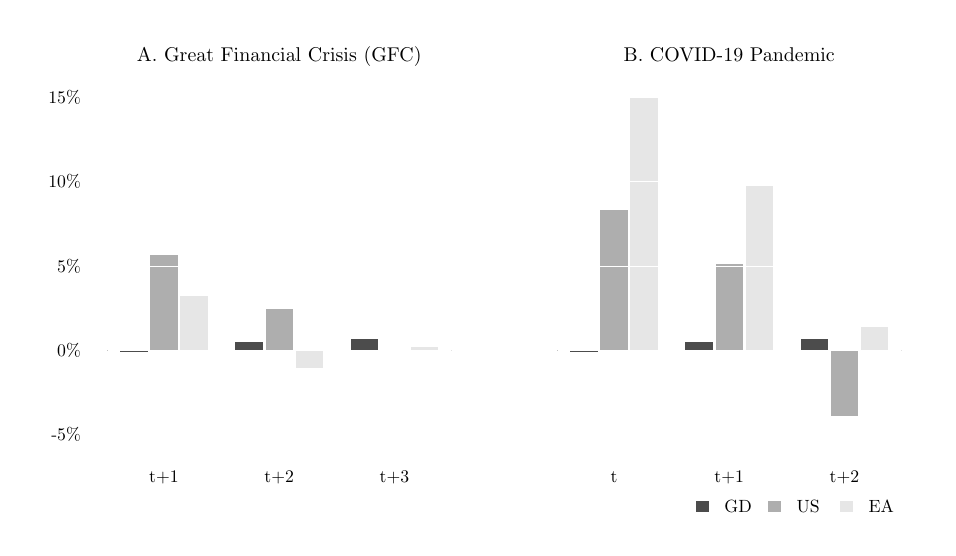
\begin{tikzpicture}[x=1pt,y=1pt]
\definecolor{fillColor}{RGB}{255,255,255}
\path[use as bounding box,fill=fillColor,fill opacity=0.00] (0,0) rectangle (325.21,180.67);
\begin{scope}
\path[clip] (  0.00,  0.00) rectangle (162.61,180.67);
\definecolor{fillColor}{gray}{0.30}

\path[fill=fillColor] ( 33.40, 64.05) rectangle ( 43.31, 63.46);
\definecolor{fillColor}{RGB}{174,174,174}

\path[fill=fillColor] ( 44.31, 64.05) rectangle ( 54.22, 98.40);
\definecolor{fillColor}{RGB}{230,230,230}

\path[fill=fillColor] ( 55.21, 64.05) rectangle ( 65.13, 83.59);
\definecolor{fillColor}{gray}{0.30}

\path[fill=fillColor] ( 75.04, 64.05) rectangle ( 84.96, 67.13);
\definecolor{fillColor}{RGB}{174,174,174}

\path[fill=fillColor] ( 85.95, 64.05) rectangle ( 95.86, 78.89);
\definecolor{fillColor}{RGB}{230,230,230}

\path[fill=fillColor] ( 96.85, 64.05) rectangle (106.77, 57.59);
\definecolor{fillColor}{gray}{0.30}

\path[fill=fillColor] (116.68, 64.05) rectangle (126.60, 68.16);
\definecolor{fillColor}{RGB}{174,174,174}

\path[fill=fillColor] (127.59, 64.05) rectangle (137.50, 63.72);
\definecolor{fillColor}{RGB}{230,230,230}

\path[fill=fillColor] (138.49, 64.05) rectangle (148.41, 65.37);
\end{scope}
\begin{scope}
\path[clip] (  0.00,  0.00) rectangle (325.21,180.67);
\definecolor{drawColor}{RGB}{0,0,0}

\node[text=drawColor,anchor=base,inner sep=0pt, outer sep=0pt, scale=  0.64] at ( 49.26, 16.32) {t+1};

\node[text=drawColor,anchor=base,inner sep=0pt, outer sep=0pt, scale=  0.64] at ( 90.90, 16.32) {t+2};

\node[text=drawColor,anchor=base,inner sep=0pt, outer sep=0pt, scale=  0.64] at (132.54, 16.32) {t+3};
\end{scope}
\begin{scope}
\path[clip] ( 28.80, 33.60) rectangle (153.01,161.47);
\definecolor{drawColor}{RGB}{0,0,0}

\path[draw=drawColor,line width= 0.4pt,line join=round,line cap=round] ( 28.80, 64.05) -- (153.01, 64.05);
\end{scope}
\begin{scope}
\path[clip] (  0.00,  0.00) rectangle (325.21,180.67);
\definecolor{drawColor}{RGB}{0,0,0}

\node[text=drawColor,anchor=base east,inner sep=0pt, outer sep=0pt, scale=  0.64] at ( 19.20, 31.40) {-5\%};

\node[text=drawColor,anchor=base east,inner sep=0pt, outer sep=0pt, scale=  0.64] at ( 19.20, 61.84) {0\%};

\node[text=drawColor,anchor=base east,inner sep=0pt, outer sep=0pt, scale=  0.64] at ( 19.20, 92.29) {5\%};

\node[text=drawColor,anchor=base east,inner sep=0pt, outer sep=0pt, scale=  0.64] at ( 19.20,122.74) {10\%};

\node[text=drawColor,anchor=base east,inner sep=0pt, outer sep=0pt, scale=  0.64] at ( 19.20,153.18) {15\%};
\end{scope}
\begin{scope}
\path[clip] ( 28.80, 33.60) rectangle (153.01,161.47);
\definecolor{drawColor}{RGB}{255,255,255}

\path[draw=drawColor,line width= 0.4pt,line join=round,line cap=round] ( 28.80, 33.60) -- (153.01, 33.60);

\path[draw=drawColor,line width= 0.4pt,line join=round,line cap=round] ( 28.80, 64.05) -- (153.01, 64.05);

\path[draw=drawColor,line width= 0.4pt,line join=round,line cap=round] ( 28.80, 94.49) -- (153.01, 94.49);

\path[draw=drawColor,line width= 0.4pt,line join=round,line cap=round] ( 28.80,124.94) -- (153.01,124.94);

\path[draw=drawColor,line width= 0.4pt,line join=round,line cap=round] ( 28.80,155.39) -- (153.01,155.39);
\end{scope}
\begin{scope}
\path[clip] (  0.00,  0.00) rectangle (162.61,180.67);
\definecolor{drawColor}{RGB}{0,0,0}

\node[text=drawColor,anchor=base,inner sep=0pt, outer sep=0pt, scale=  0.72] at ( 90.90,168.60) {A. Great Financial Crisis (GFC)};
\end{scope}
\begin{scope}
\path[clip] (162.61,  0.00) rectangle (325.21,180.67);
\definecolor{fillColor}{gray}{0.30}

\path[fill=fillColor] (196.01, 64.05) rectangle (205.92, 63.46);
\definecolor{fillColor}{RGB}{174,174,174}

\path[fill=fillColor] (206.91, 64.05) rectangle (216.83,114.88);
\definecolor{fillColor}{RGB}{230,230,230}

\path[fill=fillColor] (217.82, 64.05) rectangle (227.73,155.23);
\definecolor{fillColor}{gray}{0.30}

\path[fill=fillColor] (237.65, 64.05) rectangle (247.56, 67.13);
\definecolor{fillColor}{RGB}{174,174,174}

\path[fill=fillColor] (248.55, 64.05) rectangle (258.47, 95.19);
\definecolor{fillColor}{RGB}{230,230,230}

\path[fill=fillColor] (259.46, 64.05) rectangle (269.37,123.37);
\definecolor{fillColor}{gray}{0.30}

\path[fill=fillColor] (279.29, 64.05) rectangle (289.20, 68.16);
\definecolor{fillColor}{RGB}{174,174,174}

\path[fill=fillColor] (290.19, 64.05) rectangle (300.11, 40.23);
\definecolor{fillColor}{RGB}{230,230,230}

\path[fill=fillColor] (301.10, 64.05) rectangle (311.01, 72.50);
\end{scope}
\begin{scope}
\path[clip] (  0.00,  0.00) rectangle (325.21,180.67);
\definecolor{drawColor}{RGB}{0,0,0}

\node[text=drawColor,anchor=base,inner sep=0pt, outer sep=0pt, scale=  0.64] at (211.87, 16.32) {t};

\node[text=drawColor,anchor=base,inner sep=0pt, outer sep=0pt, scale=  0.64] at (253.51, 16.32) {t+1};

\node[text=drawColor,anchor=base,inner sep=0pt, outer sep=0pt, scale=  0.64] at (295.15, 16.32) {t+2};
\end{scope}
\begin{scope}
\path[clip] (191.41, 33.60) rectangle (315.62,161.47);
\definecolor{drawColor}{RGB}{0,0,0}

\path[draw=drawColor,line width= 0.4pt,line join=round,line cap=round] (191.41, 64.05) -- (315.62, 64.05);
\definecolor{drawColor}{RGB}{255,255,255}

\path[draw=drawColor,line width= 0.4pt,line join=round,line cap=round] (191.41, 33.60) -- (315.62, 33.60);

\path[draw=drawColor,line width= 0.4pt,line join=round,line cap=round] (191.41, 64.05) -- (315.62, 64.05);

\path[draw=drawColor,line width= 0.4pt,line join=round,line cap=round] (191.41, 94.49) -- (315.62, 94.49);

\path[draw=drawColor,line width= 0.4pt,line join=round,line cap=round] (191.41,124.94) -- (315.62,124.94);

\path[draw=drawColor,line width= 0.4pt,line join=round,line cap=round] (191.41,155.39) -- (315.62,155.39);
\end{scope}
\begin{scope}
\path[clip] (162.61,  0.00) rectangle (325.21,180.67);
\definecolor{fillColor}{gray}{0.30}

\path[fill=fillColor] (241.43,  9.57) rectangle (246.03,  5.73);
\definecolor{fillColor}{RGB}{174,174,174}

\path[fill=fillColor] (267.46,  9.57) rectangle (272.07,  5.73);
\definecolor{fillColor}{RGB}{230,230,230}

\path[fill=fillColor] (293.50,  9.57) rectangle (298.11,  5.73);
\definecolor{drawColor}{RGB}{0,0,0}

\node[text=drawColor,anchor=base west,inner sep=0pt, outer sep=0pt, scale=  0.64] at (251.79,  5.45) {GD};

\node[text=drawColor,anchor=base west,inner sep=0pt, outer sep=0pt, scale=  0.64] at (277.83,  5.45) {US};

\node[text=drawColor,anchor=base west,inner sep=0pt, outer sep=0pt, scale=  0.64] at (303.87,  5.45) {EA};

\node[text=drawColor,anchor=base,inner sep=0pt, outer sep=0pt, scale=  0.72] at (253.51,168.60) {B. COVID-19 Pandemic};
\end{scope}
\end{tikzpicture}
